% !TEX program = pdflatex

\section{Assigment 4}

\graphicspath{ {./img_presentation_4/} }
\DeclareGraphicsExtensions{.pdf,.png,.jpg}

\setlength{\fboxsep}{15pt}
\setlength{\fboxrule}{0pt}

\subsection{Application Architecture}

In the developing of the application our first focus was too keep the complexity as low as possible.

In the main interface, after the log in, the user has 3 simple main entry point:

\begin{itemize}
  \item New Booking
  \item Reservations
  \item Guests
  \item Revenue Graph
\end{itemize}

\subsubsection{New Booking}

From this entry point the user is able to add a reservation in the database.

We provide a simple and clear way to input the date periond in which book the reservation.

\fbox{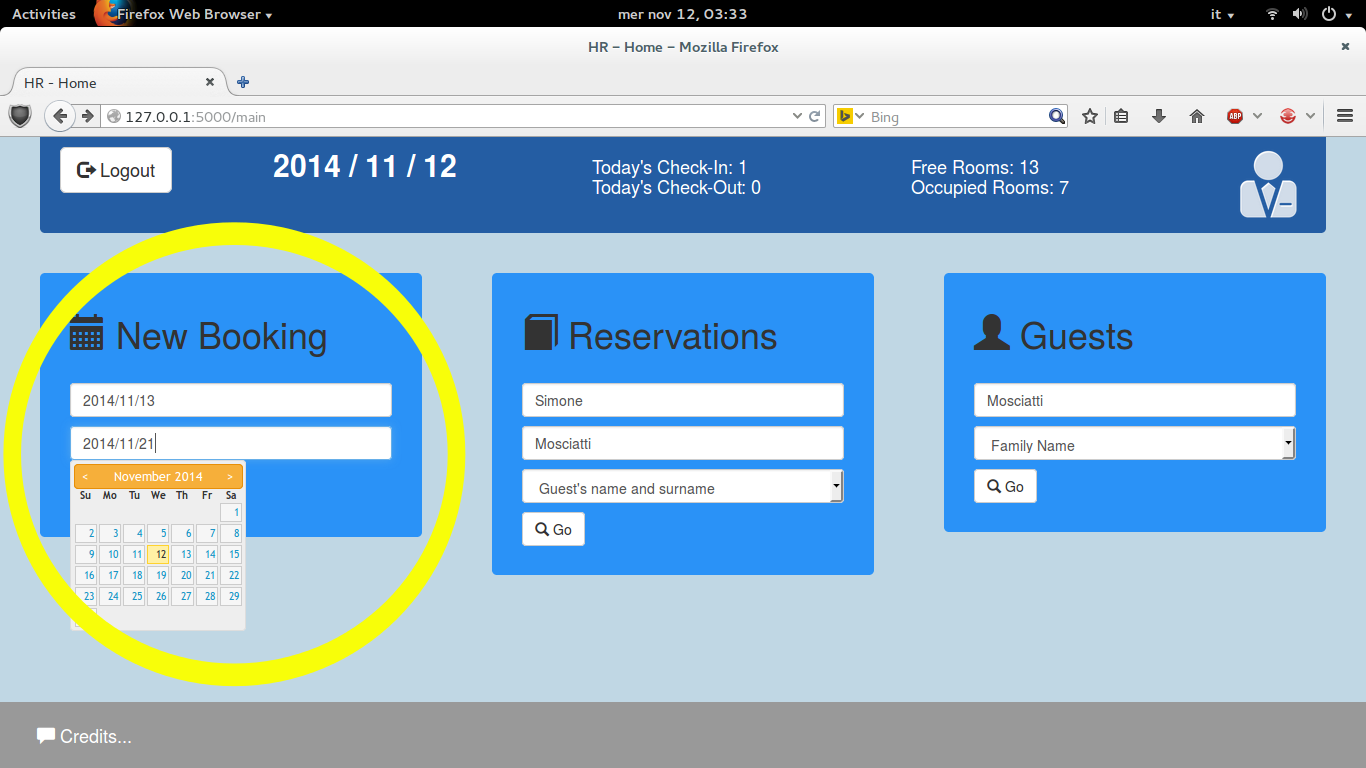
\includegraphics[width=\textwidth,height=\textheight,keepaspectratio]{show_date}}

At this point is possible to select which room associate with the guest and input the various guest information.

\fbox{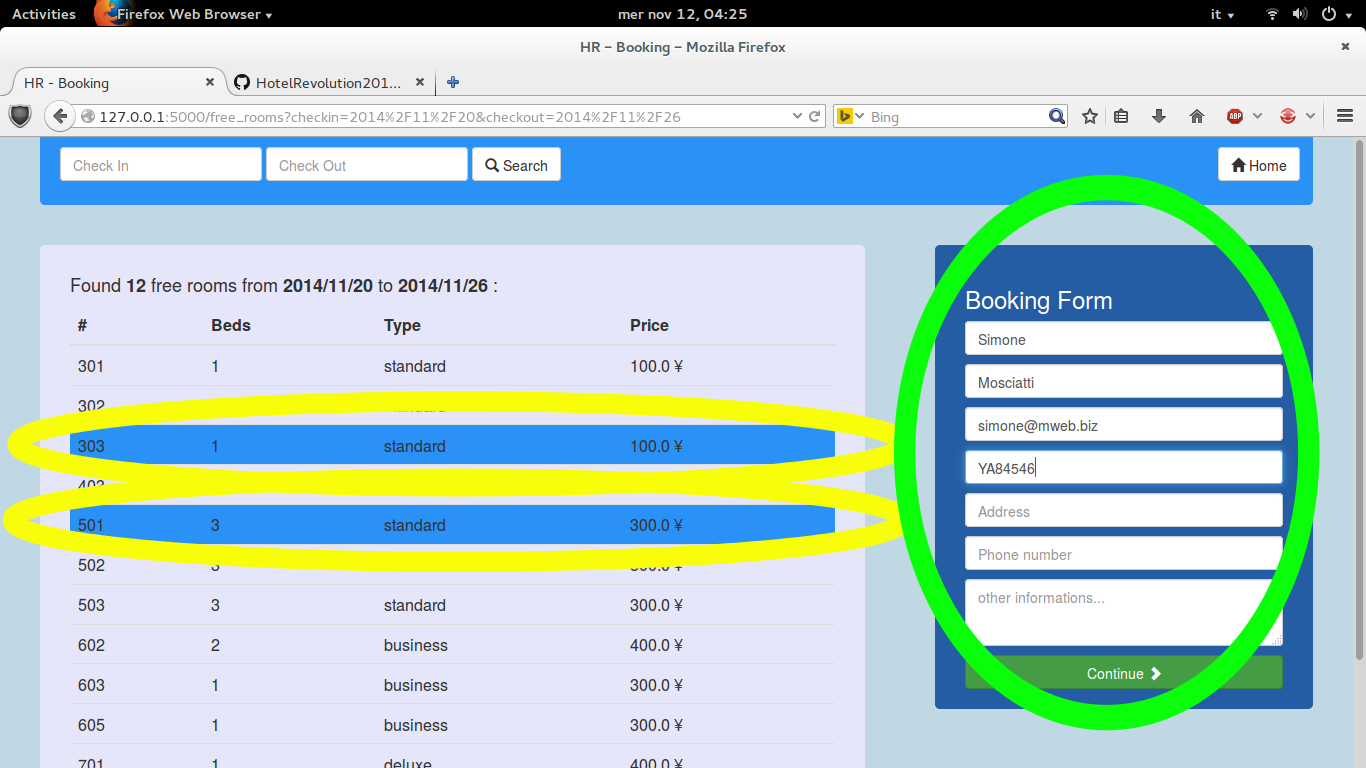
\includegraphics[width=\textwidth,height=\textheight,keepaspectratio]{select_room}}

The user is the redirect to a confirmation page where is possible to confirm the prenotation or to reject it and make other changes.

\fbox{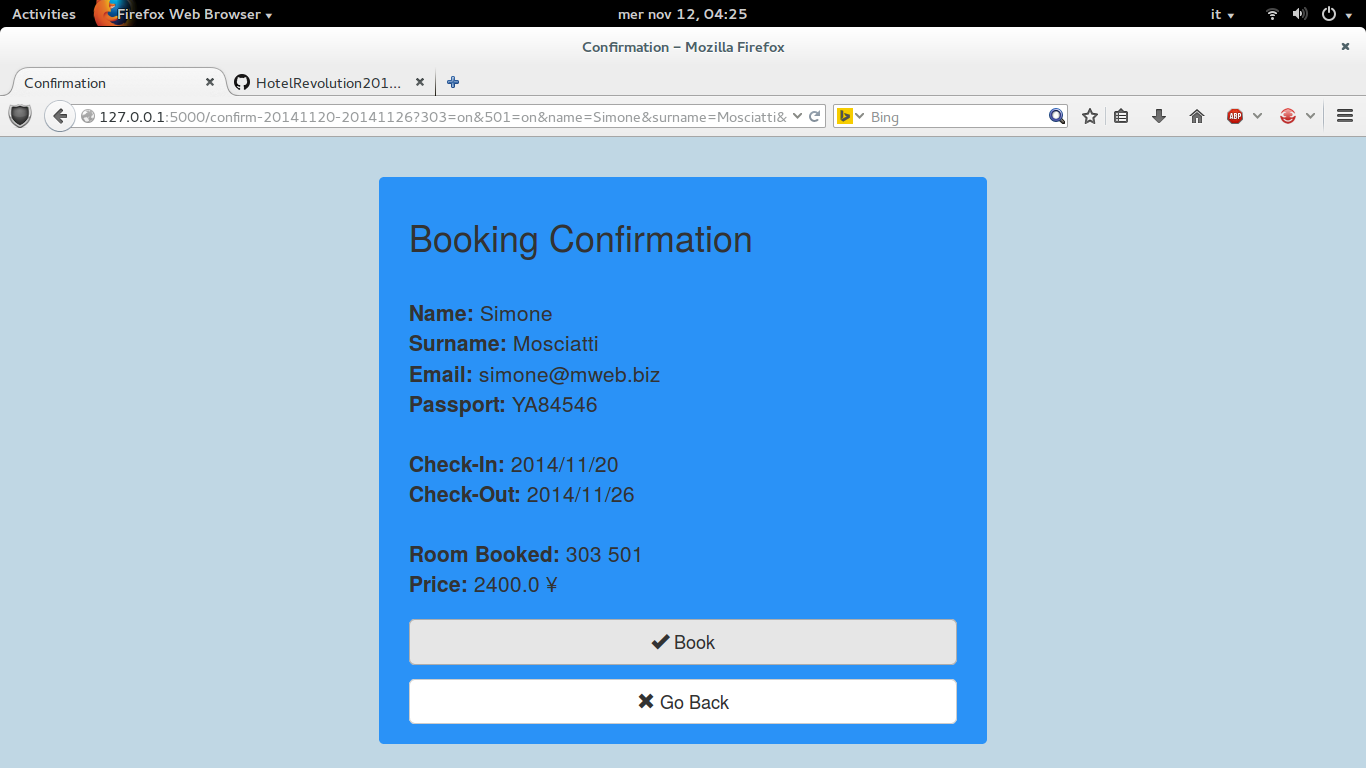
\includegraphics[width=\textwidth,height=\textheight,keepaspectratio]{confirm_booking}}

If the user reject the prenotation he will get back to the previous page.

Otherwise will be showed a small table with all the last detail of the prenotation, including the reservation ID.

\fbox{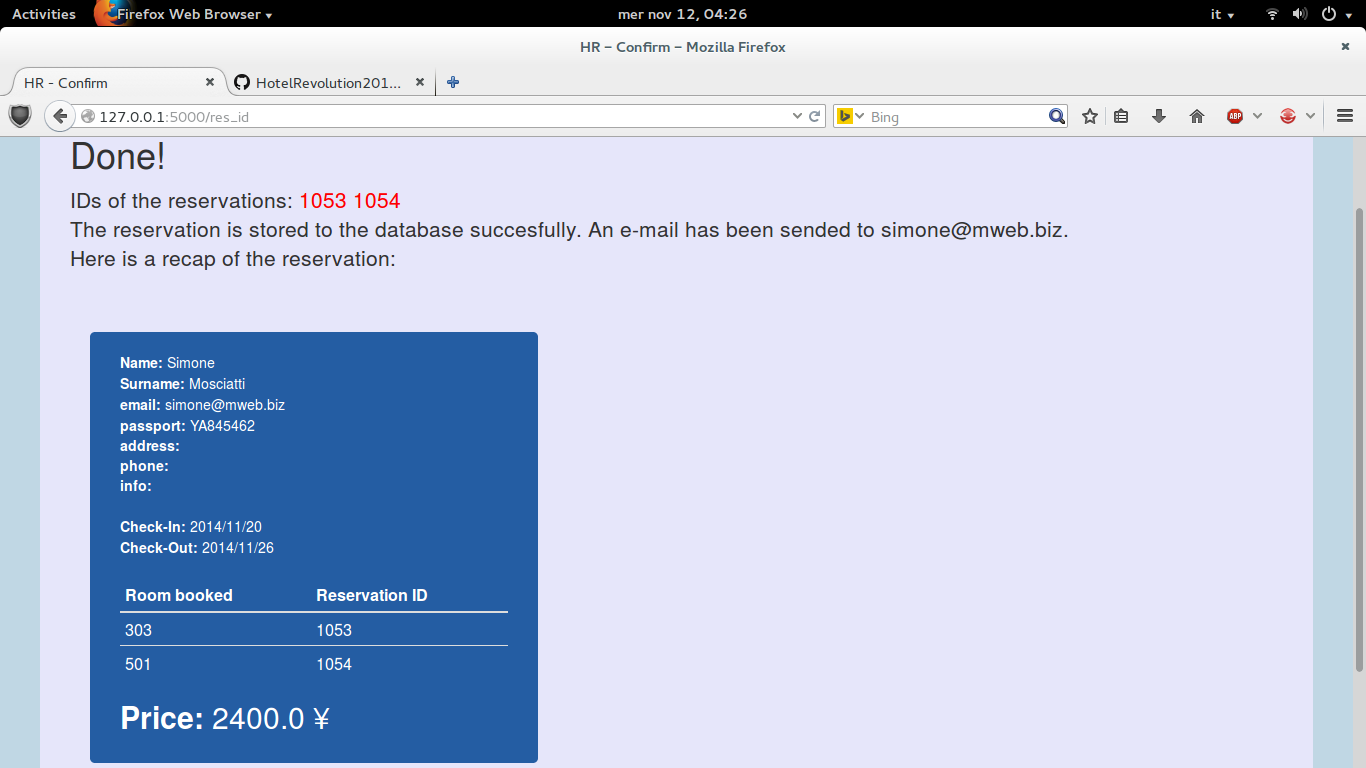
\includegraphics[width=\textwidth,height=\textheight,keepaspectratio]{confirmation}}

\subsubsection{Reservations}

This entry point enable the user to search for the reservation in the database.

It is possible to search the reservation by ID

\fbox{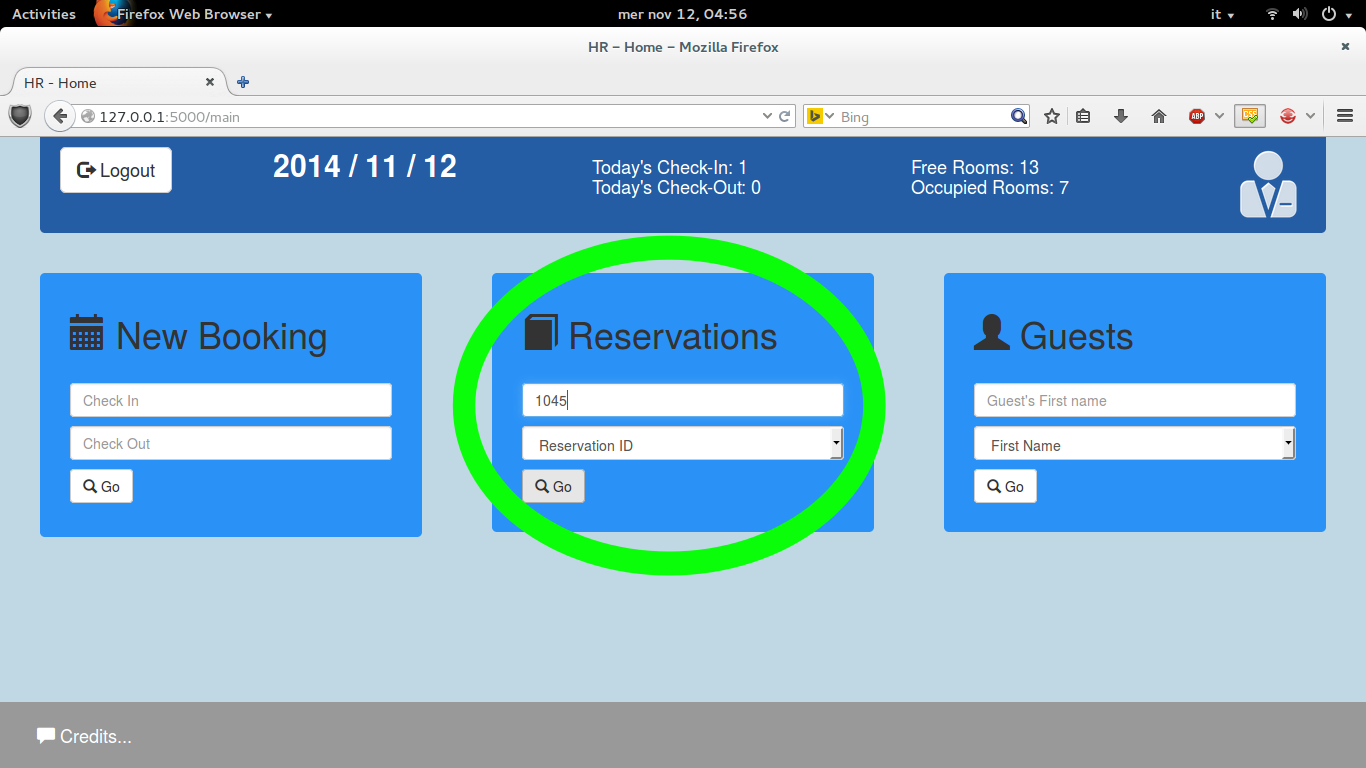
\includegraphics[width=\textwidth,height=\textheight,keepaspectratio]{id_reservation}}

or by the guest name and surname

\fbox{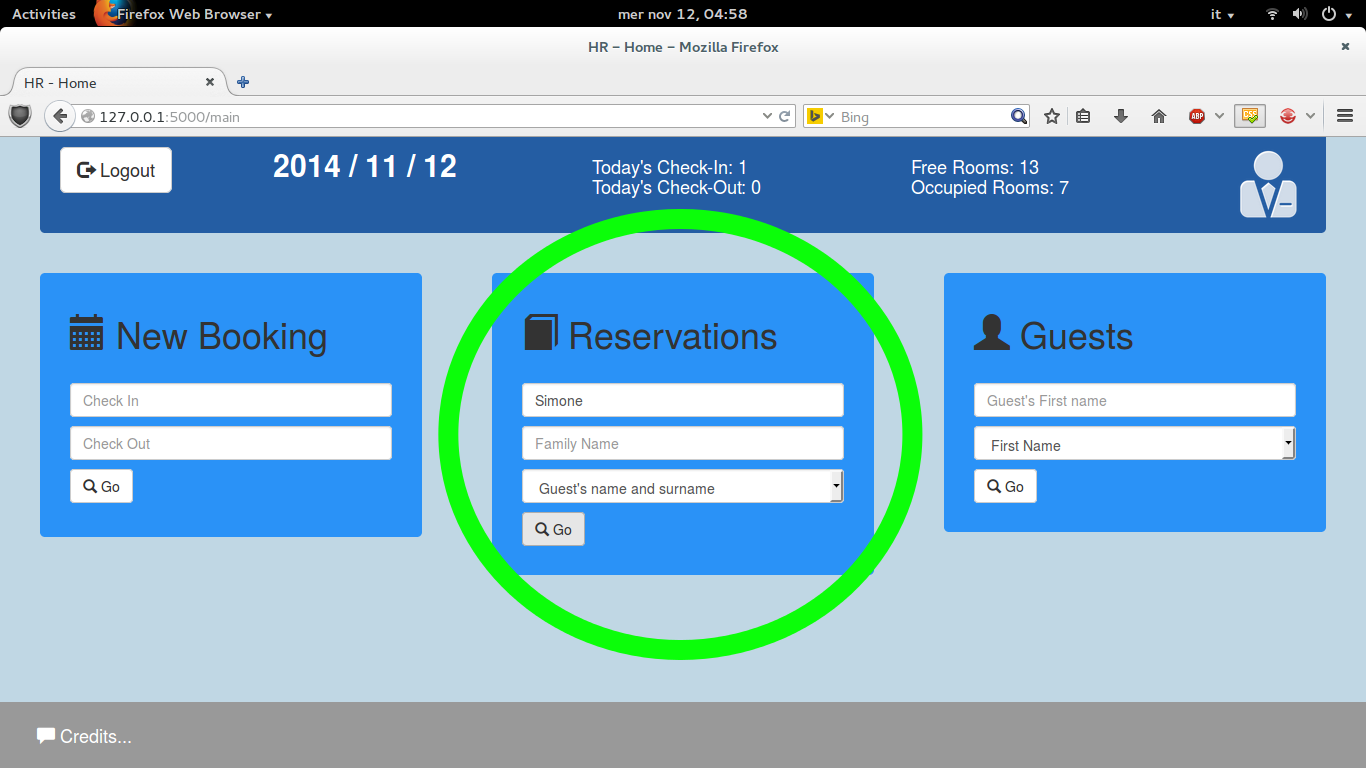
\includegraphics[width=\textwidth,height=\textheight,keepaspectratio]{name_surname_reservation}}

either research method bring to the same page

\fbox{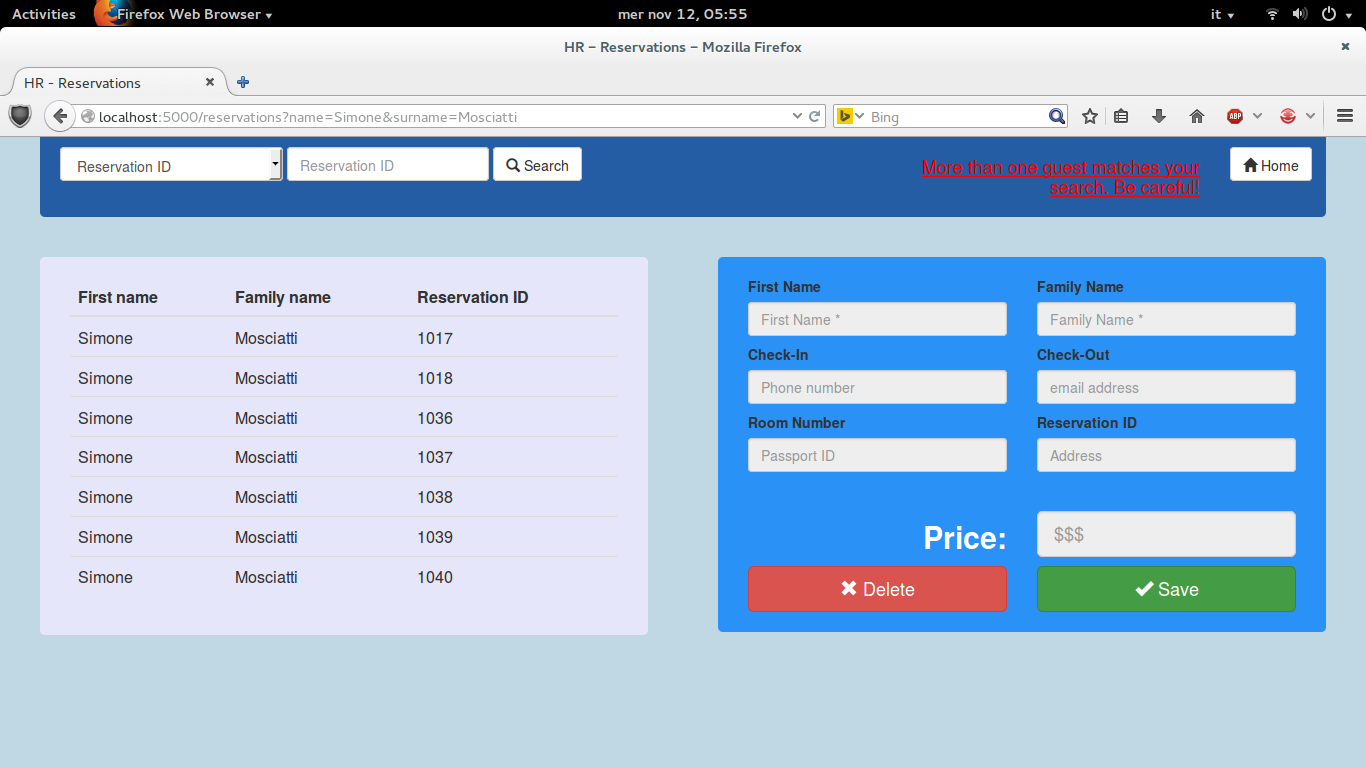
\includegraphics[width=\textwidth,height=\textheight,keepaspectratio]{show_search}}

where is possible to modify or delete a reservation.

\fbox{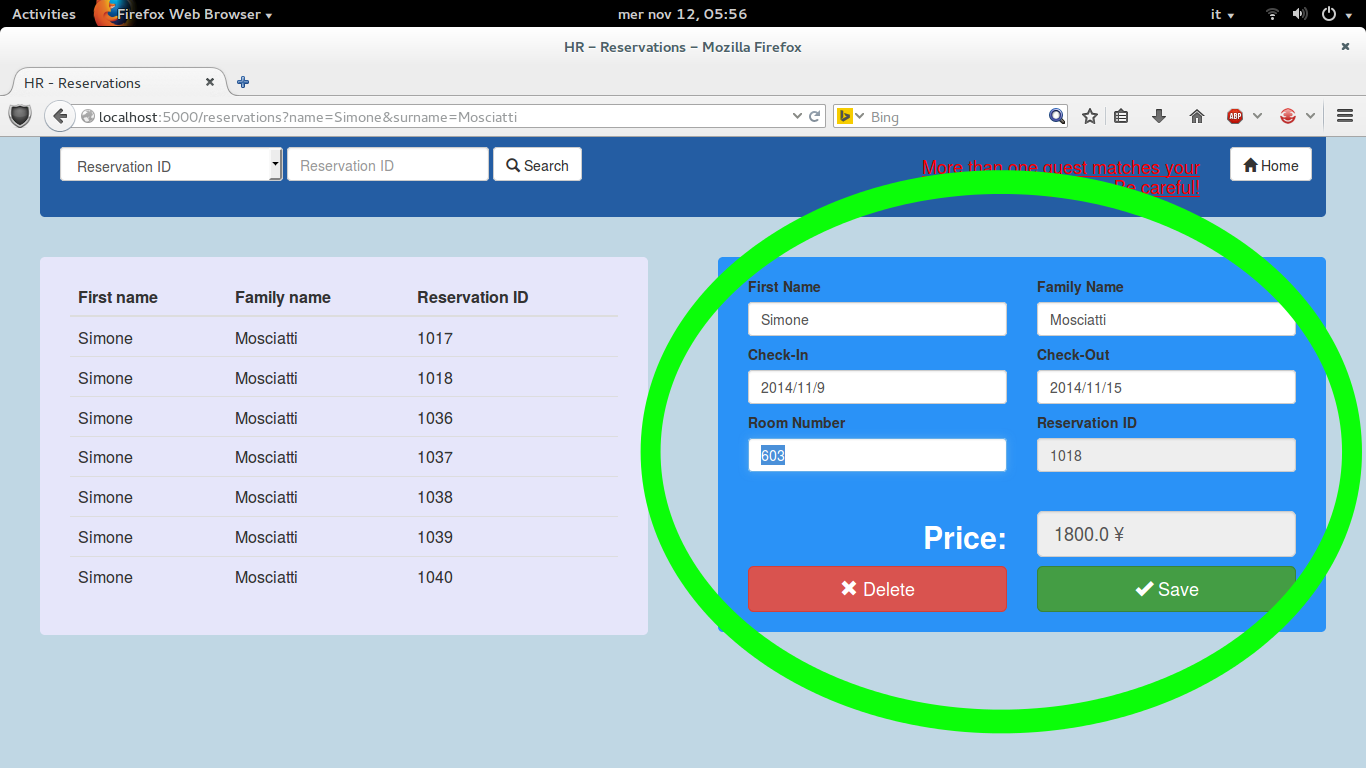
\includegraphics[width=\textwidth,height=\textheight,keepaspectratio]{change_prenotation}}

\subsubsection{Guests}

This last entry point let the user to search for the guest in the database.

It is possible to search the guest via:

\begin {itemize}
  \item First Name
  \item Family Name
  \item Passaport Number
  \item e-mail
\end{itemize}

\fbox{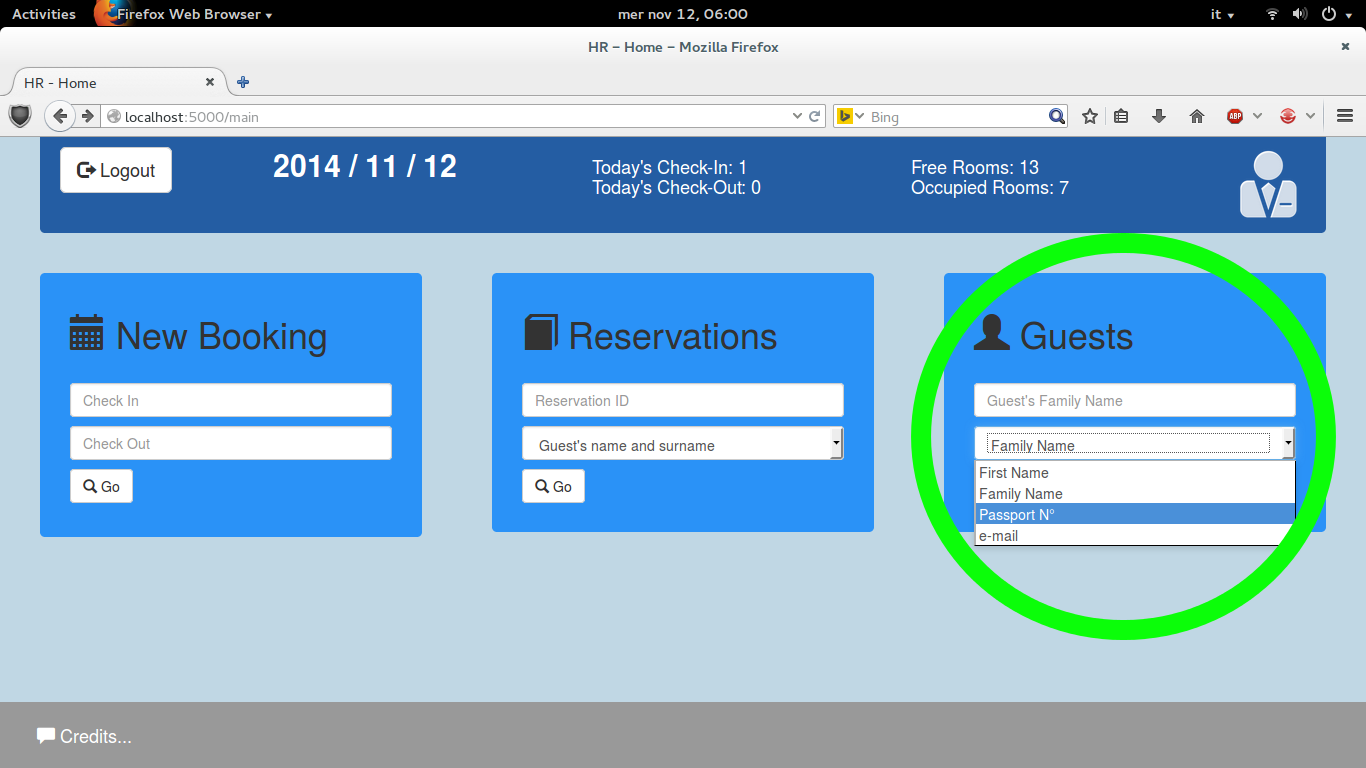
\includegraphics[width=\textwidth,height=\textheight,keepaspectratio]{search_guest}}

After the search the user is able to modify the relevant information about the guest

\fbox{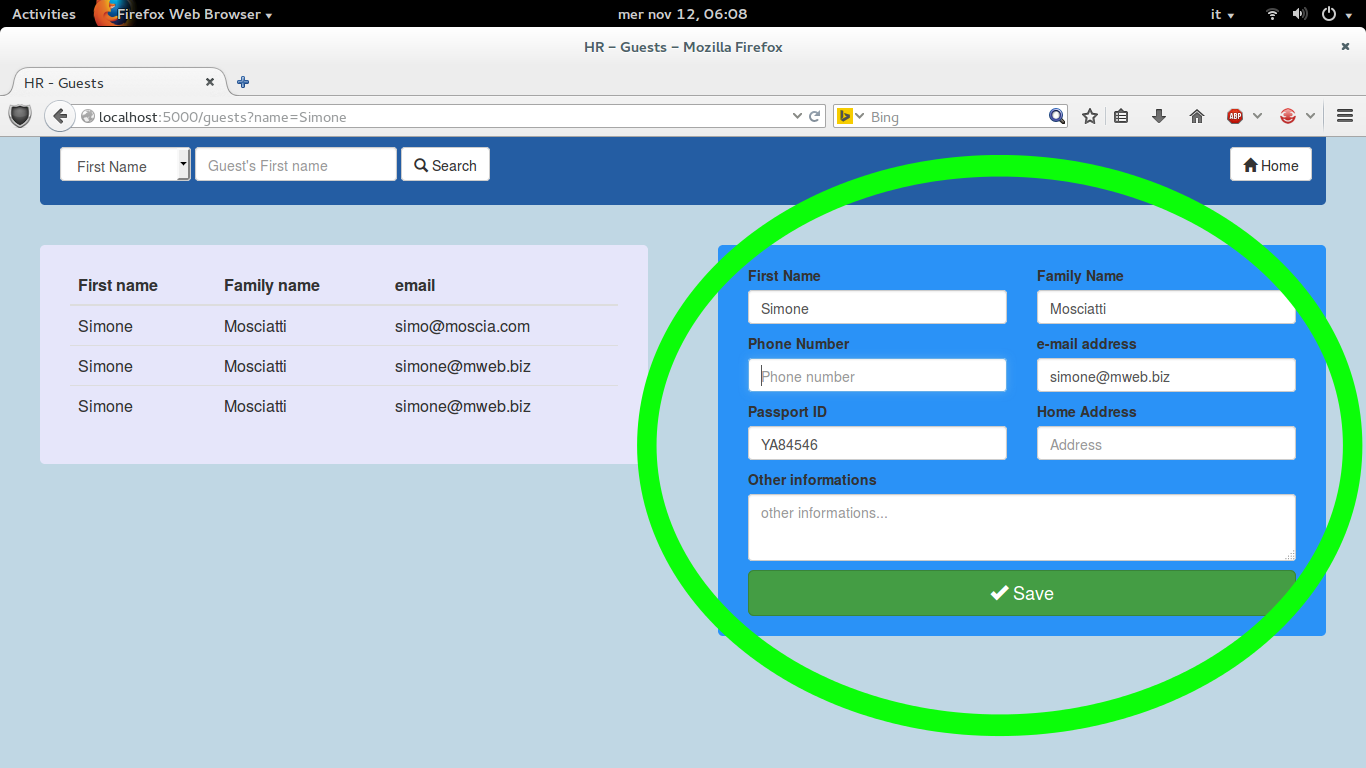
\includegraphics[width=\textwidth,height=\textheight,keepaspectratio]{modify_user_info}}

\subsubsection{Revenue Graph}

Finally, the manager have access to the revenue graph that clearly show what are the revenue of the hotel.

\fbox{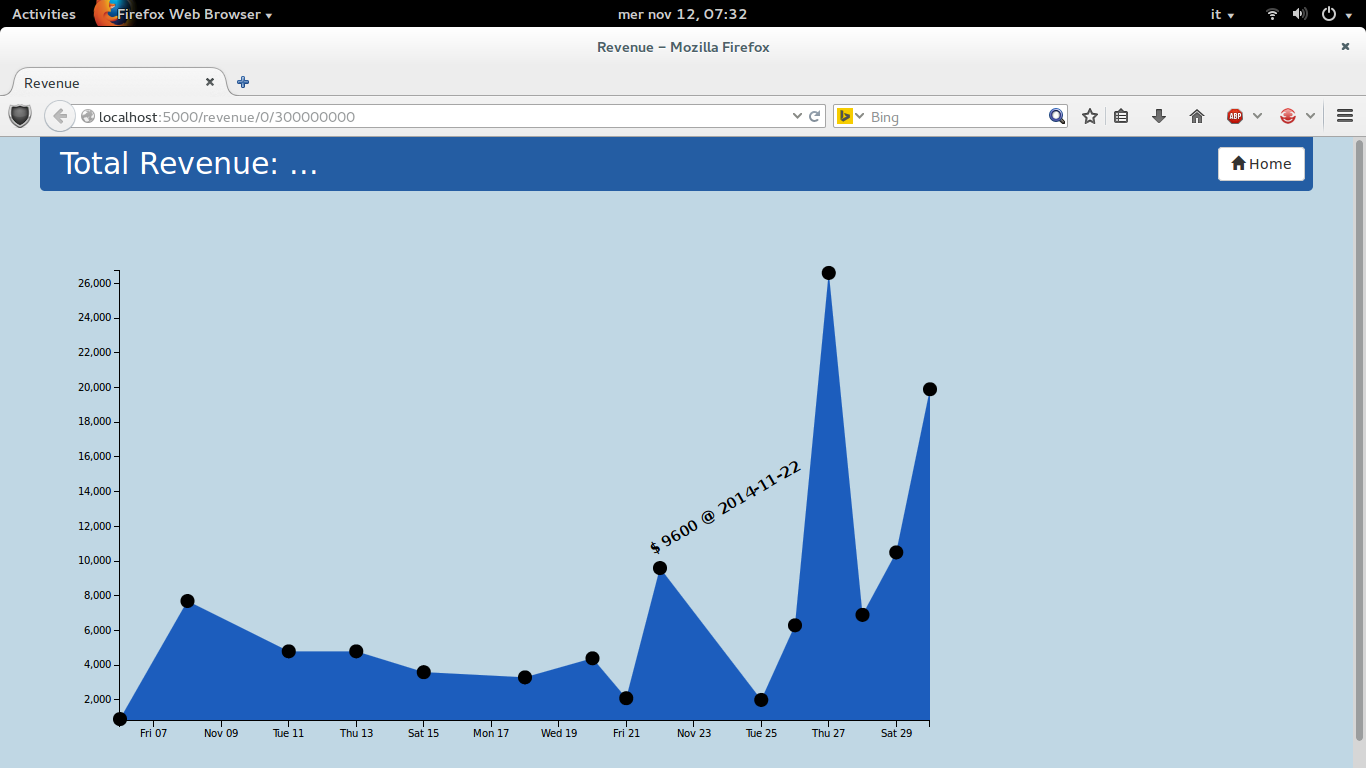
\includegraphics[width=\textwidth,height=\textheight,keepaspectratio]{graph}}

\subsection{Input Design}

\begin{center}
	\begin{longtable}{| l | l | p{7cm} |}
	\hline
	\textbf{Field Name} & \textbf{Input Type} & \textbf{Description} \\ 
	\hline \hline	
	\multicolumn{3}{|c|}{\textbf{Login}} \\ 
	\hline \hline
	Username 		& text box 		& Username \\ 
	Password 		& text box 		& Password, printed on screen like ' *** ' \\
	Log-in			& button 		& log-in if the credential are correct \\ 
	\hline \hline
	\multicolumn{3}{|c|}{\textbf{Main Page}} \\ 
	\hline \hline
	Log-out			& button		& log-out from the system and go back to the log-in \\
	Manager			& button		& go to the manager page if the user is logged as manager \\
	Credits			& button		& show in a pop-up the credits for HotelRevolution2014s \\
	\hline
	Check-in		& datepicker 	& Check-in for the new reservation \\ 
	Check-out		& datepicker 	& Check-out for the new reservation \\ 
	Booking Search	& button		& Submit a query to search a room available in the specified period (between check-in and out date \\
	\hline
	Reservation ID	& text box 		& Reservation ID \\ 
	First Name 		& text box	 	& Guest's name \\ 
	Family Name	 	& text box 		& Guest's surname \\ 
	Res Dropdown 	& dropdown 		& Switch between Reservations search method: guest's data or reservation's data \\ 
	Res Search		& button		& submit a query to search in the database the reservation the user is looking for with the previous data \\
	\hline
	Guest data		& text box		& Guest's data to search in the database, depending of the selected search method in the following dropdown \\ 
	Guest Dropdown	& dropdown 		& Switch between Guest search method: name, surname, passport, email \\ 
	Guest Search	& button		& submit a query to search the guest in the database the user is looking for with the previous data \\
	\hline \hline
	\multicolumn{3}{|c|}{\textbf{Reservations Page}} \\ 
	\hline \hline
	Reservation ID	& text box 		& Reservation ID \\ 
	First Name 		& text box	 	& Guest's name \\ 
	Family Name	 	& text box 		& Guest's surname \\ 
	Res Dropdown 	& dropdown 		& Switch between Reservations search method: guest's data or reservation's data \\ 
	Res Search		& button		& Submit a query to search in the database the reservation the user is looking for with the previous data \\
	Home			& button		& Go back to the main page \\
	\hline
	AutoFiller		& javascript	& when a row in the reservation's table is clicked, retrieve the data and fill all the text box \\
	First Name		& text box		& Guest's name for the selected reservation, retrivered from the database \\
	Family Name		& text box		& Guest's surname, as above \\
	Check-in		& text box		& Check-in, as above \\
	Check-out		& text box		& Check-out, as above \\
	Room Number		& text box		& Room number, as above \\
	Reservation ID	& text box		& Reservation Id, as above. Cannot be modified \\
	Price			& text box		& Price of the selected reservation. Cannot be modified \\
	Save			& button		& Save in the database the modified reservation's data \\
	\hline \hline
	\multicolumn{3}{|c|}{\textbf{Guests Page}} \\ 
	\hline \hline
	Guest data		& text box		& Guest's data to search in the database, depending of the selected search method in the following dropdown \\ 
	Guest Dropdown	& dropdown 		& Switch between Guest search method: name, surname, passport, email \\ 
	Guest Search	& button		& submit a query to search the guest in the database the user is looking for with the previous data \\
	Home			& button		& Go back to the main page \\
	\hline
	AutoFiller		& javascript	& when a row in the guest's table is clicked, retrieve the data and fill all the text box \\
	First Name		& text box		& Guest's name, retrivered from the database \\
	Family Name		& text box		& Guest's surname, as above \\
	email Address	& text box		& Guest's email, as above \\
	Passport ID		& text box		& Guest's passport, as above \\
	Address			& text box		& Guest's home address, as above \\
	Phone			& text box		& Guest's phone number, as above \\
	Info			& text area		& Guest's other info, as above \\
	Save			& button		& Save in the database the modified guest's data \\
	\hline \hline
	\multicolumn{3}{|c|}{\textbf{Booking Page}} \\ 
	\hline \hline
	Check-in		& datepicker	& Check-in for the new reservation \\
	Check-out		& datepicker	& Check-out for the new reservation \\
	Booking Search	& button		& Submit a query to search a room available in the written period (between check-in and out date \\
	Home			& button		& Go back to the main page \\
	\hline
	Row-selector	& checkbox		& An hidden checkbox that highlight the row and select the room for the new reservation \\
	First Name		& text box 		& Guest's first name - required input. An error occured if not filled \\
	Family Name		& text box 		& Guest's family name - required input. An error occured if not filled \\
	email Address	& text box		& Guest's email \\
	Passport ID		& text box		& Guest's passport \\
	Address			& text box		& Guest's home address \\
	Phone			& text box		& Guest's phone number \\
	Info			& text area		& If necessary, other guest's information can be written here \\
	\hline \hline
	\multicolumn{3}{|c|}{\textbf{Confirmation Page}} \\
	\hline \hline
	Book			& button		& Store the recervation into the database \\
	Go Back			& button		& If the reservation's data are not correct, go back to the booking page, where the user can modify the data \\
	\hline \hline
	\multicolumn{3}{|c|}{\textbf{Manager Page}} \\
	\hline	\hline
	Initial date	& text box		& The beginning date for calculate the revenue \\
	Final date		& text box		& The ending date for calculate the revenue \\
	Calculate		& button		& Calculate the revenue between the initial and final date \\
	Home			& button		& Go back to the main page \\
	\hline
	\end{longtable}
\end{center}

\subsection{Output Design}

According to the Hotel’s needs, outputs must be:

\begin{itemize}
  \item easy to read
  \item easy to use
\end{itemize}

So, to better meet the needs of the hotel we decide to use a tabular approach, and to organise the table in the best way possible. In order to have a quick but at the same time complete view, we decided to put only the necessary information inside the output tables. Even the columns of the tables, as you can see below, are organised in a way that consider the priority of the information required by the hotel staff. 

\begin{table}[h]
\begin{tabular}{|l|l|l|}
\hline
                    & Distribution         & Implementation Method  \\ \hline
Confirm Reservation & Receptionist - Guest & Screen - Email - Phone \\ \hline
Revenue Graph       & Manager              & Screen - Multimedia    \\ \hline
CheckOUT List       & Manager              & Screen                 \\ \hline
Reservation List    & Receptionist         & Screen                 \\ \hline
Guest List          & Receptionist         & Screen                 \\ \hline
Free Room List      & Receptionist         & Screen                 \\ \hline
\end{tabular}
\end{table}


\subsubsection{Confirm Reservation}

This Output is both internal and external. Internal because it is seen, on the screen, by the receptionist when he completes a reservation. External because it is sent by e-mail or by phone to the client. The Output design the same in both cases, and it groups the following information:
\begin{itemize}
  \item the ID of the reservation for every room that has been booked by the client
  \item the Guest e-mail
  \item all the Guest Information (name, surname, passport, address, contact, notes)
  \item the ID of every booked Room
  \item the Total Price that the guest will have to pay (i.e. the sum of the bills of every booked room)
\end{itemize}

\subsubsection{Revenue Graph}

This Output is internal and visible only by the Manager. It “prints” on the screen a detailed report of the total hotel’s revenues given a particular period of time.

The Output presents:

\begin{itemize}
  \item the total revenue of the hotel given a particular period of time and day-by-day revenues
  \item a view of the general trend of the hotel revenues
  \item a graph in which represented on the x-axis the days (of a specific period), and on the y-axis the total revenue of a particular day
\end{itemize}


\subsubsection{CheckOUT List}

This Output is a summary report, visible only by the manager, that presents a list of the checkOUT of a particular day. It prints for every room that has the checkOUT in that day the following information:

\begin{itemize}
  \item he name of the guest who booked the room
  \item the checkIN date
  \item the number of days that the room has been booked
  \item the number of the room
  \item the ID of the reservation
  \item the total price that the guest has to pay
\end{itemize}


\subsubsection{Reservation List}
This Output is an internal, and it is the result of a search in the database of the reservations. The receptionist can search and than see all the information of a reservation of a client, giving in input or the ID of the reservation, or the ID of the guest or the Name and Surname of the guest. The Output prints on the screen the following informations:

\begin{itemize}
  \item name and surname of the guest who booked the room
  \item checkIN and checkOUT dates
  \item room number of the booked room
  \item ID of the reservation
  \item total price that the client will have to pay
\end{itemize}

\subsubsection{Guest List}
This Output is internal and it is a detailed report of all informations of all guests. It prints the informations in a tabular form. Each line of the table represent a different guest:

\begin{itemize}
  \item name and surname
  \item e-mail
  \item phone number
  \item passport number
  \item address
  \item note (any particular information that the guest wants the hotel to know)
\end{itemize}

\subsubsection{Free Room List}
This is an internal Output that prints on the screen all the free room in a particular period of time. It Prints the following informations for each free room:

\begin{itemize}
  \item number of the room
  \item number of the beds of the room
  \item all the feature that are inside the room (i.e. smoker, wi-fi, …)
  \item the total price of the room for the specified period of days
\end{itemize}

\subsection{Technical Overview}

The application's backend is been developed using python and the minimalist framework ``Flask''.

We valued a lot the simplicity of the system, so we used ``SQLite'' as persintent layer.

The application's frontend is been developed using HTML and CSS, the framework ``Bootstrap'' is been used.

The HTML engine ``Jinja2'' was used to dynamically produce the desired HTML from python's data structure.

Finally the graph is render client side using the javascript library ``D3.js''.
